\chapter{基于对抗生成网络的路况图像合成技术}

\section{引言}

上一章讲到的DeepRoad测试框架在自动驾驶系统鲁棒性和稳定性测试上取得了成功,对Udacity开源的Autumn\cite{autumn},Chauffeur\cite{Chauffeur}和Rwightman\cite{Rwightman}3个自动驾驶系统都检测出了不同程度的驾驶不一致行为,展示了DeepRoad在自动驾驶系统测试工作中的价值。但是DeepRoad也有不足之处,主要问题在于:\textbf{1). }合成的自动驾驶系统测试用例,即路况图像只有雨天和雪天场景,没有覆盖到其他的天气场景,比如雾天、黄昏、夜晚等场景。 \textbf{2). }DeepRoad采用UNIT\cite{UNIT}模型来实现测试用例生成,即图像的合成转换工作,但符合人主观,图像内容清晰,内容可辨的合格图像生成率不高,实验中我们粗略地统计了一下,每1000张合成图中,可用的合格的合成图不超过50张,这极大地降低了DeepRoad测试用例自动生成的效率,也是目前DeepRoad测试框架的主要性能瓶颈。

针对上述2点问题,我们展开了对能够实现自动驾驶系统测试用例生成,即不同天气场景下路况图像合成的技术的实证研究。为了探索哪些图像合成技术能用于DeepRoad框架的测试用例生成模块,我们从DeepRoad使用的UNIT模型入手,通过文献引用,Google查询等方式对找到的每个模型进行黑盒测试,即主要关注每个模型的图像合成结果。本章主要介绍研究过程中我们先后试验过的10种不同的对抗生成网络技术,简要介绍了每个模型的实现原理以及模型技术的筛选过程以及实验数据结果样例展示,并对实验结果数据做了简要分析。

\section{基本模型与技术筛选}

\subsection{对抗生成网络的基本训练框架}

对抗生成网络\cite{GAN}首先由Ian J. Goodfellow等人提出,它的本质是模拟真实数据源的概率分布。其基本框架有两个神经网络组成:生成模型网络和判别模型网络,其中判别模型负责学习区分数据是否来自真实数据分布,而生成模型可以想象成一个制造伪币的团伙,试图产生能够通过货币监测的钞票,判别模型正是这个对抗游戏中的警察,试图甄别出货币中的假钞。整个对抗生成网络模型的训练过程就是对抗模型和生成模型的训练竞赛,整个训练过程由下图\ref{gan-wf}所示,直到判别模型再也区分不出数据是来自真实数据分布还是生成模型伪造的数据为止。

\begin{figure}[h]
    \centering
    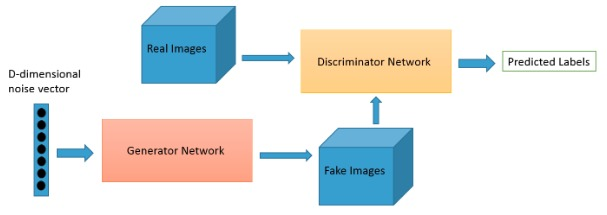
\includegraphics[width=0.8\textwidth]{gan-wf}
    \caption{对抗生成网络架构}
    \label{gan-wf}
\end{figure}

训练过程中,对抗模型一般使用向后传播算法,而判别模型一般使用向前传播算法。其中判别模型为了通过数据$x$学习生成器的数据分布$p_g$,可以基于输入的噪声数据定义一个先验概率$p_z(z)$,然后将整个数据空间表示为$G(Z;\theta_g)$,这里的$G$是一个参数为$\theta$的多层神经网络可微函数。再定义一个输出为一个单向量的多层神经元网络$D(x;\theta_d)$,其中$D(x)$表示数据$x$来自真实数据而非$p_g$的概率。我们训练$D$直到我们对所有数据正确标记其是否来自判别器的概率最大为止。同时也训练$G$来最小化$\log(1-D(G(z)))$。上述可总结成下面的公式:
\begin{equation}
    \label{eq:gan}
    \min_G\max_DV(D,G)=\xi_{x\sim p_{data}(x)}[\log D(x)]+\xi_{z\sim p_z(z)}[\log(1-D(z))]
\end{equation}

传统的对抗生成网络模型的主要缺点在与模型的训练过程很难收敛,体现在具体的实验现象上就是模型的训练很耗时,比如DeepRoad使用的UNIT模型训练一组白天-夜晚的图像转换模型,在8核1080ti GPU的硬件资源下,耗时通常在一周左右,普遍高于其它一般的深度学习模型训练时长。对抗生成网络难收敛的主要原因有3点:1. 实际训练过程中,等式\eqref{eq:gan}中的生成器$G$可能会出现梯度消失的问题;2. 判别器$D$的损失函数一般为KL散度函数,文献\cite{arj}表明该函数在训练过程中很容易导致不收敛。

\subsection{风格数据集的扩充与预处理}

虽然之前DeepRoad工作中使用爬虫技术从Youtube视频网站上收集一定量的风格数据集,但主要是雨天和雪天场景,我们希望还能够实现除此外其他场景的风格转换,比如黄昏、夜晚等场景,因此我们在原有的数据集上又收集了几个国外大学以及研究组织提供的开源路况数据集:Oxford RobotCar\cite{ds:oxford},Comma.ai\cite{ds:ai},Berkeley大规模自动驾驶视频数据集\cite{ds:berkeley}。其中Oxford RobotCar和Berkeley数据集中很多图像中包含了Udacity数据集中没有的元素,比如雨天场景下的汽车雨刷,由于摄像头位于汽车内驾驶室靠后位置而出现的车窗框,驾驶员等与路况信息无关的噪声信息。我们对含有此类噪声的图像进行了人工的排查和去除。

\subsection{模型筛选}

从文献\cite{UNIT}入手,通过文献引用,以及文献\cite{gan-survey}的调研,我们发现目前主流的对抗生成网络变种技术有以下几类:1). \textbf{全连接对抗生成网络},即模型中的生成器和判别器都有全连接网络构成,具体实现为Goodfellow最初提出的原生GAN模型。这类模型主要应用在一些相对简单的图像数据集上,比如MNIST,CIFAR-10等。2). \textbf{卷积对抗生成网络},虽然卷积神经网络在图像的特征表示上有天然的优势,但由于梯度消失的现象会导致训练很难收敛,文献\cite{LAPGAN}中提出多尺度对抗生成网络训练框架,文献中给出的实验数据显示多尺度的生成器能加速模型训练的收敛,一定程度上缓解了模型的慢收敛问题。采用此类结构的具体技术最典型的为DCGAN\cite{dcgan}。3). \textbf{条件对抗生成网络},传统的对抗生成网络对于输入的随机噪声数据会呈现除不稳定状态,导致生成的数据与需求难以匹配,针对该问题,条件对抗生成网络由于对多模型分布的数据有更好的表征能力,于是能一定程度上地解决此问题,他通过对生成器和判别器模型加入条件变量来模拟随机噪声数据分布。该类模型典型的技术实现有cGAN\cite{cGAN}。4). \textbf{变分自编码对抗生成网络},自动编码器是由编码器和解码器构成的网络,能够将数据映射到潜在表征空间内,它的主要优点在于不仅能够想卷积神经网络一样很好的实现图像识别功能,还能实现将图像内容的内容元素和风格元素拆分,并分别映射到潜在内容空间和风格空间上,利用来自不同内容空间和风格空间的元素合成新的图像。这类模型的典型技术实现有WGAN\cite{WGAN}。

\begin{figure}[h]
    \centering
    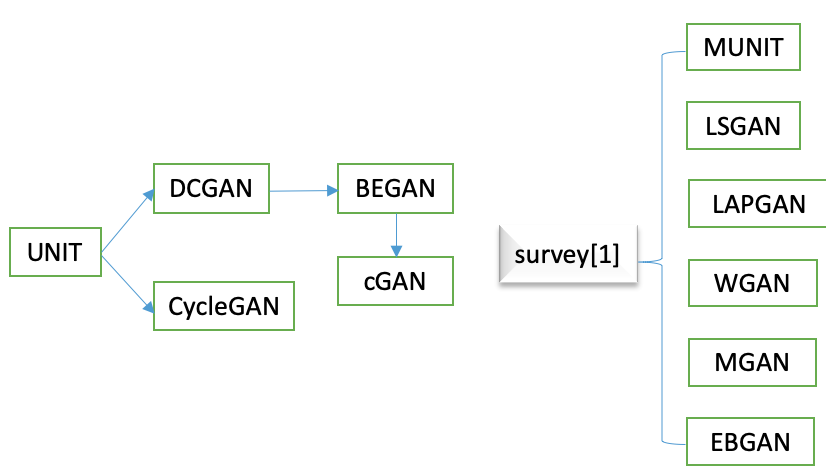
\includegraphics[width=.6\textwidth]{gan-filter}
    \caption{对抗生成网络模型收集}
    \label{gan-filter}
\end{figure}

本工作中针对可实现图像变换功能的对抗生成网络技术的收集过程如图\ref{gan-filter}
所示。由于实验中的各种原因,诸如文献提供源代码作者放弃了代码维护导致实验重现困难,部分模型对训练数据集十分敏感,导致将实验数据集换成自制数据集后,实验结果,即合成图像质量效果太差等因素我们对实验的模型进行了淘汰筛选工作。下面对研究过程中实验过的模型依次进行简要的介绍。

\subsubsection{cGAN}

\textbf{cGAN.}\cite{cGAN}\quad 对抗生成网络一般有两个对抗模型组成:一个可以捕捉到真实数据分布的生成模型$G$和一个能够计算样本来自训练数据集而不是$G$的概率的模型$D$。$D$和$G$都是非线性映射函数,比如多层感知器网络。如果生成器和判别器都限定于一些额外信息$y$上,则对抗生成网络可以被拓展成一个条件模型。其中$y$可以使任意类型的辅助信息,比如来自其他模型的数据或标记。cGAN通过将数据信息$y$送入判别器和生成器中作为额外的输入层来实现条件限制。在生成器中先验噪声输入$p_z(z)$和$y$被混合在联合隐藏层中,在判别器中$x$和$y$代表判别函数的输入,cGAN的目标函数可以表示为:
\begin{gather}
    min_G max_D V(D,G)=\mathbb{E}_{\x\sim p_{data}(x)}[\log D(x|y)]+\mathbb{E}_{z\sim p_z(z)}[\log(1-D(G(z|y)))]
\end{gather}

因为文献中\cite{cGAN}主要对MNIST\cite{mnist}数据集进行了数字模拟合成,在已有的路况图像数据集上实验的结果很不理想,图\ref{fig:cgan}为cGAN的实验结果样例图,我们简单分析实验结果不理想的主要原因在与cGAN使用的是一个浅层卷积神经网络,学习能力有限,对一些语义信息比较简单的图像有很好的特征提取性能,但对复杂的图像,比如我们使用的路况图像,则不能很好的学习到图像的高级特征,导致最后的合成图效果很差,因而我们放弃了在该模型上的进一步实验与数据统计。 

\begin{figure}[h]
    \centering
    \includegraphics[width=.24\textwidth]{models/cGAN/1}
    \includegraphics[width=.24\textwidth]{models/cGAN/2}
    \includegraphics[width=.24\textwidth]{models/cGAN/3}
    \includegraphics[width=.24\textwidth]{models/cGAN/4}
    \caption{cGAN实验结果样例图}
    \label{fig:cgan}
\end{figure}

\subsubsection{DCGAN}[DCGAN]

\textbf{DCGAN.}\cite{dcgan}\quad 是一个深度卷积对抗生成网络,其生成器和判别器使用的是限制卷积网络,主要的架构特点有:(1)用多步卷积和分布卷积层代替了所有的池化层(pooling layer);(2)使用了批量统一化层(batch normalization layer);(3)去掉了所有的全连接层;(4)在生成器中,使用$\tan{h}$作为输出层的激活函数,ReLU函数作为其它层的激活函数;(5)判别器中,所有层的激活函数都使用LeakyReLU函数。除此之外该算法结构中,所有正定空间池化函数都换成了多步卷积函数,这样可以使网络网络学习到整个图像空间的采样。

DCGAN主要目的是找到一个方法能够对图像进行特征重建及特征提取。DCGAN在其卷积神经网络的拓扑结构内提出了一套限制,使得该模型能够几乎在任何参数设置里都能够尽快的训练收敛。相较其他的对抗生成网络模型,DCGAN的主要优点是其稳定的网络结构和较快的训练收敛速度。DCGAN的作者将该模型在CIFAR-10\cite{cifar10}数据集上做了一次实证研究,结果也验证了DCGAN较其他GAN模型能够更快的学习到图像的特征。

虽然DCGAN的作者将其运用在人脸合成与转换上相当成功,但我们后来将其训练集换成了Udacity的自动驾驶路况数据集以及youtube上爬取的数据,实验结果样本图如下图\ref{dcgan_example}所示,效果不理想。

\begin{figure}[h]
    \centering
    \includegraphics[width=\textwidth]{models/DCGAN/1}
    \caption{DCGAN实验结果样例图}
    \label{dcgan_example}
\end{figure}

实验过程中,我们参考了\cite{dcgan}论文中给出的算法,针对我们收集的路况图像数据集调整了部分网络结构和训练参数,具体配置参数如下

\begin{lstlisting}[basicstyle=\small]
    --bathSize     200          // 批量实验数据大小
    --imageSize    180, 320     // 设置图像尺寸大小
    --nz           20           // z向量
    --niter        10000        // 训练的次数
    --lr           0.0002       // Learning rate
    --cuda                      // 在cuda库上训练
\end{lstlisting}

由于DCGAN在驾驶路况图片上的合成效果很差,于是我们放弃了对该框架进一步的实验结果数据统计与总结。

\subsubsection{LAPGAN}

\newmodel{LAPGAN} 该模型利用了图像的多尺度结构,针对每个尺度构建了一系列的生成模型,每个模型都在特定尺度的拉普拉斯算子\cite{lapcode}上捕获到了图像的结构特征。这种方法将原来的图像转换问题成功地分解成了一系列可控状态,对于每个状态都可以使用一般的对抗生成网络结构训练一个基于卷积神经网络的生成模型。

在视觉应用,比如目标分类中的判别模型中,使用深度学习的方法常常十分有效。但是对于生成模型,尽管进行了相当多的研究\cite{lapgan1}\cite{lapgan2}\cite{lapgan3},却往往没有取得同等级别的成功。基于这样的问题,LAPGAN提出了模型在生成模型的训练效果上取得了巨大的改进。模型中使用的拉普拉斯算子是由一组图像的线性非可逆表征组成。具体的,使$d(\cdot)$表示模糊化$i\times j$图像$I$的缩减采样算子,则$d(I)$表示尺度为$j/2\times l/2$的新图像。类似地,令$u(\cdot)$表示将图像$I$光滑化的升采样算子,$u(I)$表示尺度为$2j\times 2j$的新图像。算法中首先构建一个高斯拉普拉斯算子$\mathbb{G}(I)=[I_0,I_1,\dots,I_K]$,这里的$I_0=I$和$I_k$表示$d(\cdot)$对$I$的$k$次重复操作。$K$是该算子中的层数。拉普拉斯网络中每一层$k$的系数$h_k$都是由邻近层中的距离计算构成,对图像使用算子$u(\cdot)$进行升采样操作:
\begin{gather}
    h_k=\mathbb{L}_k(I)=\mathbb{G}(I)-u(\mathbb{G}_{k+1}(I))=I_k-u(I_{k+1})
\end{gather}
每层都很直观的包含了特定尺度的图像结构信息。拉普拉斯算子$h_k$的最终结构是一张不同的图像。以此为基础可成功的重构一张新图像。

该算法文献\cite{LAPGAN}中在CIFAR10数据集上进行了图像转换实验,但实验的代码没有进行开源,因此我们暂时性的忽略了该算法的实验。将来该算法代码开源后我们会针对该算法进行补充实验和数据统计。 

% wc ~ 1200

\subsubsection{CycleGAN}[CycleGAN]

\textbf{CycleGAN.}\cite{CycleGAN}\quad 该模型的本质是学习不同图片类(比如晴天和雨天)的数据分布映射函数。给定两个不同类的数据集$X$和$Y$以及训练样本集$\{x_i\}_{x=1}^N, \{y_j\}_{j=1}^M$,其中$x_i\in X, y_j\in Y$。将数据分布记为$x\sim p_{data}(x), y\sim p_{data}(y)$。如图\ref{lable-cyclgan}所示,CycleGAN包含两个映射函数$G: X\to Y$和$F: Y\to X$,其次,CycleGAN还引进了两个判别器$D_X$和$D_Y$,其中$D_X$的目标是区分图像集$\{x\}$和转换的图像集$\{F(y)\}$,同样的,$D_Y$的目标是区分图像集$\{y\}$和$\{G(x)\}$。最终模型的训练目标是得到两个损失函数:(i)对抗损失函数,可以将合成的图像数据分布匹配对应到目标类的数据分布上;(ii)循环一致损失函数,阻止之前学习到的两个映射函数$G$和$F$彼此相矛盾。

\begin{figure}[h]
    \centering
    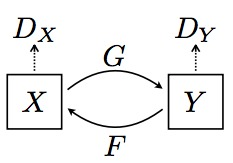
\includegraphics[width=.35\textwidth]{cyclegan_1}
    \caption{CycleGAN}
    \label{lable-cyclgan} 
\end{figure}

CycleGAN将对抗损失应用到了两个映射函数上,对于映射函数$G:X\to Y$和他的判别器$D_Y$,可以将其目标函数表示为
\begin{equation}
\begin{aligned}
    \label{eq:2}
    L_{GAN}(G,D_Y,X,Y)= & \xi_{y\sim p_{data}(y)}[\log D_Y(y)] + \\
    & \xi_{x\sim p_{data}(x)}[\log (1-D_Y(G(x)))]
\end{aligned}
\end{equation}

这里的$G$试图产生类似于类$Y$的图像集$G(x)$,然而$D_Y$的目标是区分转换的图像$G(x)$和真实的图像数据$y$。$G$旨在与对抗器$D$竞争最小化该目标函数。

对抗器理论上可以训练出可以输出和目标类$Y$与$X$分布完全相同的数据的映射函数$G$和$F$,但是如果网络的体积足够大,可以将相同的输入图片集映射到目标图片类的任意图像子集里。因此,单靠对抗损失函数无法保证学习到了映射函数能将单张输入图片$x_i$映射到理想的输出$y_i$。为了进一步减小可能的映射函数空间,CycleGAN提出循环一致映射函数,即对于来自类$X$的每张图像,对应的图像转换循环应该能够将$x$转换成原始图片,即\textit{向前循环一致}。上述的循环一致损失函数可以表示为:
\begin{equation}
\begin{aligned}
    \label{eq:3}
    L_{cyc}(G,F)= & \xi_{x\sim p_{data}(x)}[||F(G(x))-x||_1] + \\
    & \xi_{y\sim p_{data}(y)}[||G(F(y))-y||_1]
\end{aligned}
\end{equation}

综合等式\ref{eq:2}和等式\ref{eq:3}我们可以得到总的目标函数:
\begin{equation}
\begin{aligned}
    L(G, F, D_X, D_Y) = & L_{GAN}(G,D_Y, X, Y) \\
    & + L_{GAN}(F,D_X, Y, X) \\
    & + \lambda L_{cyc}(G, F)
\end{aligned}
\end{equation}
这里的$\lambda$控制着两个目标的相对重要性。

CycleGAN对于内容图片通训练图片不相似的情况转换合成效果并不好,常常会造成合成图的语义不明确。它通常适合于颜色和图像纹理转换的情形,对于合成图有内容变化的情形,CycleGAN合成图的效果会比较差,其作者分析其中的原因可能是因为常常会为了提高图像信息变化更高效而裁减生成器的网络复杂度,这使得CycleGAN对于内容改变的性能变差。文献\cite{CycleGAN}中也提到了CycleGAN对于一组不相似的图片训练出来的模型效果较一组相近训练数据集模型效果会差很多,并且很难消除这两者间的差异。

图\ref{fig:cyclegan}是我们将CycleGAN运用在我们的数据集上的实验结果样本图。 

\begin{figure}[h]
    \centering
    % \subfigure[原始图片]{
    %     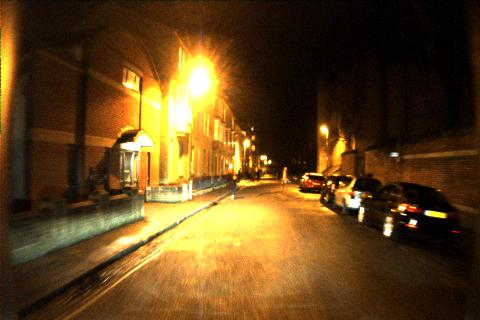
\includegraphics[width=0.3\textwidth]{results/cyclegan-input}
    % }
    % \subfigure[白天场景]{
    %     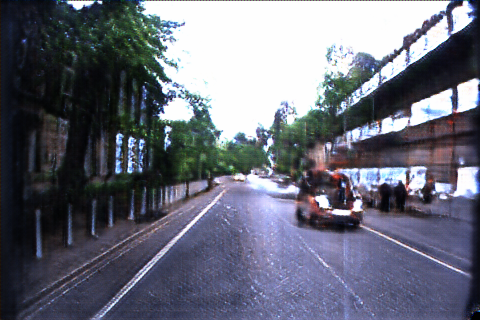
\includegraphics[width=0.3\textwidth]{results/cyclegan-sun}
    % }
    % \subfigure[黑天场景]{
    %     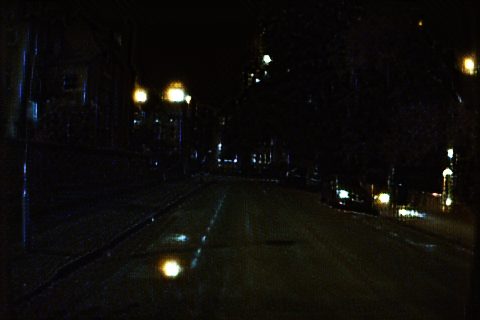
\includegraphics[width=0.3\textwidth]{results/cyclegan-night}
    % }
    % \subfigure[官方样例-1]{
    %     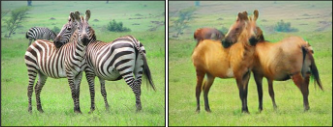
\includegraphics[width=0.45\textwidth]{cyclegan_o_1}
    % }
    % \subfigure[官方样例-2]{
    %     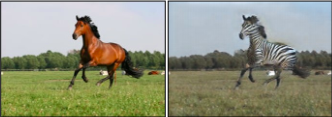
\includegraphics[width=0.45\textwidth]{cyclegan_o_2}
    % }

    \includegraphics[width=.24\textwidth]{models/CycleGAN/1}
    \includegraphics[width=.24\textwidth]{models/CycleGAN/2}
    \includegraphics[width=.24\textwidth]{models/CycleGAN/3}
    \includegraphics[width=.24\textwidth]{models/CycleGAN/4}
    \includegraphics[width=.24\textwidth]{models/CycleGAN/5}
    \includegraphics[width=.24\textwidth]{models/CycleGAN/6}\includegraphics[width=.24\textwidth]{models/CycleGAN/7}
    \includegraphics[width=.24\textwidth]{models/CycleGAN/8}
    \caption{CycleGAN实验样例图}
    \label{fig:cyclegan}
\end{figure} 

% wc ~ 800

\subsubsection{WGAN}

\newmodel{WGAN} 该算法相较其他的GAN模型的主要改进依然是提升了模型训练的稳定性和收敛速度。WGAN提出了Earth-Mover距离,并证明了该距离比其他的距离尺度指标能产生更好的梯度,从而提升训练速度。此外它关于判别器网络还去掉了对应了sigmoid层,在对抗损失函数中去掉了log函数,有效地避免的类似模型塌缩等问题。理论上图像合成的效果要好于DCGAN。

因为WGAN文献中只给出了算法的核心思想,没有给出实验源码。我们参考文献中提供的算法,实现了WGAN的图像转换代码,但是在路况图像数据集上的实验结果十分不理想,合成的图像与原图像在语义上相差甚远,我们猜测可能是算法实现没有成功导致,最终我们没有将该实验结果纳入最后的实验数据总结和统计中。图为Udacity白天到雪天场景的转换样例图。

\begin{figure}[ht]
    \centering
    \includegraphics[width=\textwidth]{models/WGAN/1}
    \caption{WGAN实验样例图}
    \label{fig:wgan}
\end{figure}

\subsubsection{MUNIT}[MUNIT]

\textbf{MUNIT.}\cite{MUNIT}\quad MUNIT是基于UNIT\cite{UNIT}工作的进一步优化。它主要针对的问题时候多类图像间的图像转换问题。比如一个冬天的道路场景在夏天可能会依天气、时间等因素的不同而有很多种不同的外在形式。CycleGAN希望其生成器能够包含一个场景中尽可能多的表征空间。

除此之外它提出了一个可以解决多模型图片到图片转换问题的框架。它对于图像转换问题提出了几个假设:图片的潜在空间(latent space)可以被分解成内容空间和样式空间。基于上一个假设又提出了不同域类的图片共享一个类似的内容空间,但样式空间不一致。为了将一张图片转换成目标域类,MUNIT提出可以将图片的内容码与目标域类样式码空间的一个随机样式码重组。这里的内容码代表了在图片转换过程中应该被保留的信息元,而状态码则代表了不包含在输入图片中还剩下的变量元。通过采样不同的状态码,MUNIT模型能够产生多样,多模型的输出。以上严格的数学定义如下:

\begin{figure}[t]
    \centering
    \includegraphics[width=\textwidth]{models/MUNIT/1}
    \caption{MUNIT实验样例图}
    \label{fig:munit}
\end{figure}

假定$x_1\in \chi_1$和$x_2\in \chi_2$是来自两个图片域类的图片集,给定来自两个不同边缘分布$p(x_1)$和$p(x_2)$的样本图片集,但不知道联合分布$p(x_1, x_2)$。MUNIT的目的是利用学习到的图片到图片转换模型$p(x_{1\to 2}|x_1)$和$p(x_{2\to 1}|x_2)$来预测两个边缘分布$p(x_1|x_2)$和$p(x_2|x_1)$,这里的$x_{1\to 2}$是由将$x_1$转换成$x_2$产生的一个样本输出。一般来说,$p(x_1|x_2)$和$p(x_2|x_1)$通常是十分复杂且多模型分布,为了简化这两个边缘分布,MUNIT提出了\textit{部分共享潜在空间假设}。即假设每张图片$x_i\in \chi_i$都是由两种码,内容码和样式码,组成,其中内容码$c\in C$由两个类域共享,而样式码$s_i\in S_i$则是每个域类图片所特有的。换句话说,一组来自联合分布的对应的图片$(x_1, x_2)$是由$x_!=G_1^*(c,s_1)$和$x_2=G_2^*(c, s_2)$生成的,这里的$c,s_1,s_2$都是来自鲜艳分布,$G_1^*,G_2^*$是实际的生成器。进一步假设$G_1^*$和$G_2^*$是确定性函数,且有反解码器$E_1^*=(G_1^*)^{-1}$和$E_2^*=(G_2^*)^{-1}$。MUNIT的目的是利用神经网络学习实际的生成器以及编码函数。它使用了两个重建的目标函数:给定来自数据分布的图像样本,在编码和解码后我们能够重建它:
\begin{gather}
    L_{recon}^{x_1}=E_{x_1\sim o(x_1)}[||G_1(E_1^c(x_1), E_1^s(x_1))-x_1||_1] 
\end{gather}

给定在转换时的样式和内容码,我们也应该能够在解码和编码后重建图像:
\begin{equation}
    \begin{aligned}
        L_{recon}^{c_1}= & E_{c_1\sim p(c_1), s_2\sim q(s_2)}[||E_2^c(G_2(c_1,s_2))-c_1||_1] \\
    L_{recon}^{s_2}= & E_{c_1\sim p(c_1), s_2\sim q(s_2)}[||E_2^s(G_2(c_1, s_2))-s_2||_1]
    \end{aligned}
\end{equation}

结合以上公式,MUNIT的总的损失函数可以由下面的公式表示:
\begin{equation}
\begin{aligned}
    \min_{E_1,E_2,G_1,G_2}\max_{D_1,D_2}L(E_1,E_2,G_1,G_2,D_1,D_2)=L_{GAN}^{x_1}_L_{GAN}^{x_2}+\\
\lambda_x(L_{recon}^{x_1}+L_{recon}^{x_2})+\lambda_c(L_{recon}^{c_1}+L_{recon}^{c_2})+\lambda_s(L_{recon}^{s_1}+L_{recon}^{s_2})
\end{aligned}
\end{equation}

总体来说,MUNIT是一个多模型无监督图像到图像的转换框架。在目前的无监督方法中图像转换质量和转换图像的种类都更好更多。最后我们使用了MUNIT提供的代码,进行了晴天路况图和雪天场景的转换,主要的优化配置参数如下,最终的实验结果样例及MUNIT官方实验样例图参考图\ref{fig:munit}:

\begin{lstlisting}[basicstyle=\small, caption={MUNIT主要优化参数配置}, captionpos=b]
    max_iter: 1000000             # maximum number of training iterations
    batch_size: 1                 # batch size
    weight_decay: 0.0001          # weight decay
    beta1: 0.5                    # Adam parameter
    beta2: 0.999                  # Adam parameter
    init: kaiming                 # initialization [gaussian/kaiming/xavier/orthogonal]
    lr: 0.0001                    # initial learning rate
    lr_policy: step               # learning rate scheduler
    step_size: 100000             # how often to decay learning rate
    gamma: 0.5                    # how much to decay learning rate
    gan_w: 1                      # weight of adversarial loss
    recon_x_w: 10                 # weight of image reconstruction loss
    recon_s_w: 1                  # weight of style reconstruction loss
    recon_c_w: 1                  # weight of content reconstruction loss
    recon_x_cyc_w: 10             # weight of explicit style augmented cycle consistency loss
    vgg_w: 0                      # weight of domain-invariant perceptual loss
\end{lstlisting}

\subsubsection[EBGAN]{EBGAN}

\textbf{EBGAN.}\cite{ebgan}\quad 的核心思想是将判别器视为一个能量函数而不是通常的概率函数。它构建了一个函数能将输入空间中的每个点映射成为一个单标量,并且提出了对抗生成模型训练的一个基于能量表达的公式。由判别器计算出来的能量函数可以被视作生成器的可训练代价函数。虽然可以将能量函数通过Gibbs分布转换成概率函数,但是基于它提出的基于能量形式的对抗生成网络由于缺少归一化,从而使我们在判别器的架构和训练过程中有了更多的选择。EBGAN的学习构成是由数据驱动,定型能量函数是的好的模型参数配置获得低能量而不好的配置参数获得高能量。这种训练书序监督学习的一种:对于每训练集中的每个$X$,一种$(X,Y)$的能量只有当$Y$是好的配置参数时才会获得低能量,反之获得高能量。下面简单阐述一下EBGAN的基本原理。

将$p_{data}$视作产生真实数据集分布的概率密度函数,生成器$G$训练生成赝本数据$G(z)$。为了定义能量函数,判别器的输出通过一个目标泛函算子进行转换,将低能量视为真实样本数据,而高能量则为合成的伪数据。跟一般的对抗生成网络一样,EBGAN也使用了两个不同的损失函数来分别训练生成器和判别器。

给定一个正边缘分布函数$m$,一个数据样本$x$和一个生成样本$G(z)$,判别器损失函数$L_D$和生成器损失函数$L_G$可以定义为以下:
\begin{equation}
    \begin{align*}
    L_D(x, z) = & D(x) + [m - D(G(z))] \\
    L_G(z) = & D(G(z))
    \end{align*}
\end{equation}

给定一个生成器$G$,$p_G$为$G(z)$的密度分布,这里$z\sim p_z$。换句话说,$p_G$是由$G$产生的样本的概率密度函数。定义$V(G,D)=\int_{x,z}L_D(x,z)p_{data}(x)p_z(z)dxdz$和$U(G,D)=\int_zL_G(z)p_z(z)dz$,训练中判别器来最小化$V$值,生成器最小化$U$值。该系统的纳什均衡是一组满足一下条件的一对$(G^*,D^*)$:
\begin{equation}
    \begin{aligned}
        V(G^*,D^*) \leq V(G^*,D) \quad\quad \forall D \\
        U(G^*,D^*) \leq U(G,D^*) \quad\quad \forall G 
    \end{aligned}
\end{equation}

EBGAN打通了两类不同的非监督学习方法:对抗生成网络和自动编码器,并且从基于能量的角度重新采用对抗生成网络的结构并定义新的训练损失函数。对于高分辨率图片,相较其他类的对抗生成网络技术,EBGAN的模型训练有更快的收敛速度,且合成图片也有更好的合成效果。

我们在已有的数据集上使用tensorflow库实现了晴天路况到雨天和夜晚场景的转换,图\ref{fig:ebgan}是实验结果样例图。

\begin{figure}[ht]
    \centering
    \includegraphics[width=.24\textwidth]{models/EBGAN/1}
    \includegraphics[width=.24\textwidth]{models/EBGAN/2}
    \includegraphics[width=.24\textwidth]{models/EBGAN/3}
    \includegraphics[width=.24\textwidth]{models/EBGAN/4}
    \includegraphics[width=.24\textwidth]{models/EBGAN/5}
    \includegraphics[width=.24\textwidth]{models/EBGAN/6}
    \includegraphics[width=.24\textwidth]{models/EBGAN/7}
    \includegraphics[width=.24\textwidth]{models/EBGAN/8}
    \caption{EBGAN实验样例图}
    \label{fig:ebgan}
\end{figure}

\subsubsection{LSGAN}

\newmodel{LSGAN} 一般的GAN模型都使用sigmoid交差熵作为判别器的损失函数,使用这类损失函数都存在一个问题,就是在模型训练过程中很容易出现梯度消失的问题,导致最后合成的数据离真实数据分布相差较大。针对这一问题LSGAN提出使用最小方差函数最为判别器的损失函数,因为最小方差损失函数能够使判别器对接近判断边界的伪数据做出惩罚。除此之外,LSGAN还能提高模型训练过程的稳定性。文献\cite{LSGAN}提到实验结果显示LSGAN合成的数据别一般的GAN合成输数据更接近与真实数据分布。该算法的目标损失函数为:
\begin{equation}
\begin{aligned}
    & \min_D V_{LSGAN}(D)=\frac{1}{2}\mathbb{E}_{x\sim p_{data}(x)}[(D(x)-b)^2]+\frac{1}{2}\mathb{E}_{z\sim o_z(z)}[(D(G(z))-z)^2] \\
    & \min_G V_{LSGAN}(G)=\frac{1}{2}\mathb{E}_{z\sim p_z{z}}[(D(G(z))-c)^2]
\end{aligned}
\label{con:f1}
\end{equation}

\begin{figure}[h]
    \centering
    \includegraphics[width=\textwidth]{models/LSGAN/1}
    \caption{LSGAN合成图像对比图}
    \label{fig:lsgan}
\end{figure} 

因为文献\cite{LSGAN}中算法使用的网络结构跟DCGAN\cite{dcgan}使用的非常接近,主要区别在于损失函数的差别,于是我们使用Pytorch实现了公式\ref{con:f1}中的损失函数,训练算法以及网络架构代码都沿用DCGAN的代码,实验结果如图\ref{fig:lsgan}所示,我们发现合成图质量与DCGAN相差无几,质量提升不大,主要原因可能是公式\ref{con:f1}使用的损失函数不适用与路况图像的合成。基于较差的实验结果我们舍弃了该模型实验结果的数据统计和总结。

\subsubsection{MGAN}

\newmodel{MGAN} 大部分用于图像合成的对抗生成网络技术都是使用马尔可夫随机场来处理图像复杂的限制特征,这些马尔可夫随机场也通常是使用像素块的统计数据来表征图像的。这类技术通常分为两类:合成完整图像的全图像模型和只合成图像纹理层的马尔科夫模型。MGAN主要的改进是提升了深度马尔科夫模型对纹理合成的效率与质量。文献\cite{MGAN}中使用对抗训练\cite{adtrain}算法训练卷积神经网络,这样可以维持与原图几乎不变的图片质量,同时极大地提升了图像合成速度,40ms内合成一张$512\times 512$图像,其中硬件条件为TitanX GPU。

因为MGAN的优化主要针对人脸合成类别,且与传统的图像合成技术类似,合成图片具有明显的艺术风格。我们利用文献中提供的代码\cite{git:mgan}在我们的路况图像数据集上实验结果跟文献中的实验结果一致,具有太明显的艺术风格,因而在最后的实验数据统计和总结环节我们没有考虑该模型的实验数据。下图\ref{fig:mag}为MGAN的实验数据样例图。

\begin{figure}[h] 
    \centering
    \includegraphics[width=.23\textwidth]{models/MGAN/1}
    \includegraphics[width=.23\textwidth]{models/MGAN/2}
    \includegraphics[width=.23\textwidth]{models/MGAN/3}
    \includegraphics[width=.23\textwidth]{models/MGAN/4}
    \includegraphics[width=.23\textwidth]{models/MGAN/5}
    \includegraphics[width=.23\textwidth]{models/MGAN/6}
    \includegraphics[width=.23\textwidth]{models/MGAN/7}
    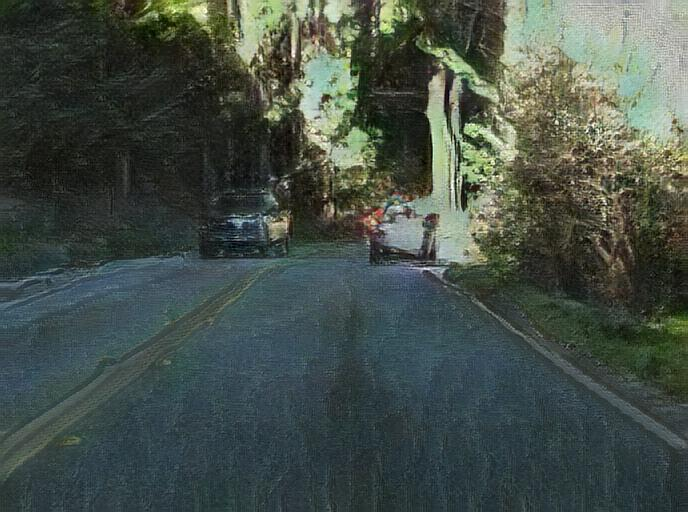
\includegraphics[width=.23\textwidth]{models/BEGAN/21}
    \caption{MGAN实验样例图}
    \label{fig:mag}
\end{figure}

\subsubsection{BEGAN}

\newmodel{BEGAN}  该模型跟EBGAN\cite{ebgan}一样使用了自动编码器作为判别器。虽然一般典型的对抗生成网络模型都直接匹配数据分布,但是BEGAN的目的是利用从Wasserstein距离中推到出了损失函数,来匹配自动编码器损失值。分布。实际的模型算法中,使用了一个典型的对抗生成网络目标函数,加上一个额外的平衡判别器和生成器的平衡因子。这样使得模型的训练更加容易。文献\cite{BEGAN}中对于自动编码器使用的损失函数$\mathb{L}:\mathbb{R}^{N_x}\to \mathbb{R}^+$为:
\begin{align}
    \mathb{L}(v) = |v-D(v)|^\eta where \begin{cases}
        D: \mathbb{R}^{N_x}\to \mathbb{R}^{N_x} \quad  \\
        \eta \in \{1,2\} \quad  \\
        v \in \mathbb{R}^{N_x} 
    \end{cases}
\end{align}

模型总体的目标函数可表示为:

\begin{align}
    \begin{cases}
        L_D = L(x) - k_t\cdotL(G(z_D)) & for \quad \theta_D \\
        L_G = L(G(z_G)) & for \quad \theta_G \\
        k_{t+1} = k_t + \lambda_k(\gammaL(x)-L(G(z_G))) 
    \end{cases}  
\end{align}

我们参考了文献中的代码\cite{BEGAN}实现了WGAN的人脸图像合成,但将数据源换成我们的路况图像数据集后,发现合成的图像质量效果太差,图\ref{fig:began}为实验结果样例图,基于时间成本考虑我们放弃了对该模型的进一步实验和数据统计。

\begin{figure}[h]
    \centering
    \includegraphics[width=.23\textwidth]{models/BEGAN/1}
    \includegraphics[width=.23\textwidth]{models/BEGAN/2}
    \includegraphics[width=.23\textwidth]{models/BEGAN/3}
    \includegraphics[width=.23\textwidth]{models/BEGAN/4}
    \includegraphics[width=.23\textwidth]{models/BEGAN/5}
    \includegraphics[width=.23\textwidth]{models/BEGAN/6}
    \includegraphics[width=.23\textwidth]{models/BEGAN/7}
    \includegraphics[width=.23\textwidth]{models/BEGAN/8}
    \caption{BEGAN人脸合成样例图}
    \label{fig:began}
\end{figure} 

\section{总结}

我们通过文献查询等各种方式找到上述10种能实现图像风格变换的对抗生成网络技术后,试图对每种模型技术都进行路况图像的风格转换实验,但由于其中的cGAN,LSGAN,LAPGAN没有将使用的代码开源,除此外,BEGAN、WAGN和MGAN技术文献中给出的代码由于原作者已放弃了维护,我们试图运行过各个技术官方给出的代码,发现上诉模型代码都存在各种BUG,比如使用过于老的第三方库,代码定制无法扩展到其他数据集,经过实验成员的讨论,已经时间成本的考虑,我们放弃了对以上模型技术的进一步实验。最后成功得到实验数据的有DCGAN、CycleGAN、EBGAN、cGAN、MUNIT、LSGAN和LAPGAN。

\subsection{实验结果统计与分析}

实验中我们的内容图像集统一使用Udacity的晴天路况图像集,在将风格图像集替换成前文介绍的各个开源数据集后并开展了图像风格转换实验后我们发现大部分模型的最后实验效果都太差了,比如图\ref{bad-res}展示了利用cGAN进行晴天到晚上场景的路况图像转换结果样例图。

\begin{figure}[h]
    \centering
    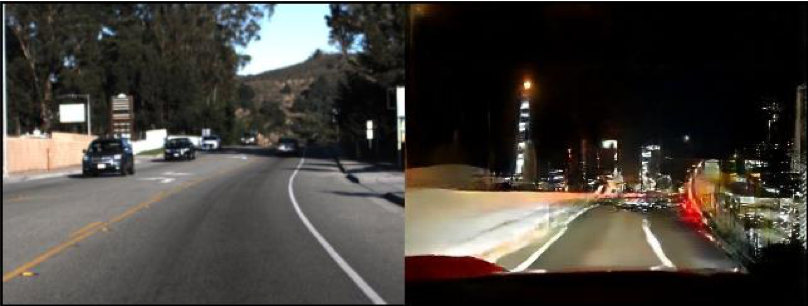
\includegraphics[width=0.4\textwidth]{bad1}
    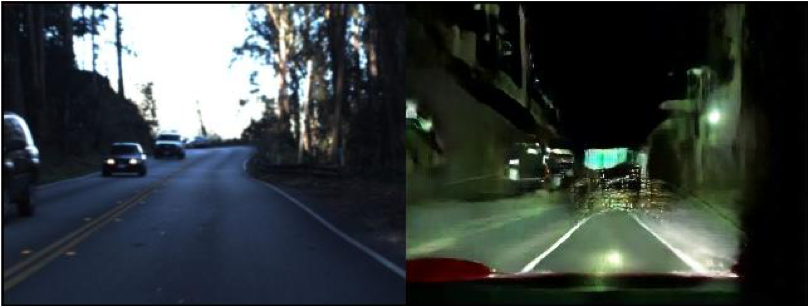
\includegraphics[width=0.4\textwidth]{bad2}
    \caption{cGAN实验结果样例图}
    \label{bad-res}
\end{figure}

对于此类技术,我们认为实验结果,即合成图质量过于不真实,对DeepRoad测试框架中测试用例合成模块的使用价值不大,因为即便使用不真实的图像检测出了监视系统的不一致行为,我们很难探明出现的不一致行为的原始是自动驾驶系统的缺陷,还是合成图与真实图相差太大导致的,并且形如图\ref{bad-res}中展示的合成图在现实场景中也不可能出现,所以将他们放入自动驾驶系统的测试集中也没有意义。基于以上原因,我们放弃了对DCGAN、cGAN、LSGAN和LAPGAN实验结果数据的进一步统计和分析。最终我们成功实验,并对实验结果数据进行了统计和总结的模型有:MUNIT、CycleGAN和EBGAN。

对于cGAN、CycleGAN等模型合成图效果太差的原因我们也做了简要的分析,可能的原因在于DCGAN、cGAN、LSGAN和LAPGAN的技术实现中,对于生成器都使用了变分自编码技术,使用编码器将图像集投射到内容空间和风格空间上,然后再利用解码器对拥有不同风格的图像集基于各自的内容空间和风格空间的码元进行重组,从而实现图像的风格变换,这种技术有明显的缺陷,即如果两组图像的内容和风格相差太大,则使用互相的内容空间和风格空间里的码元进行图像重构,得到的输出会因本身图像集之间的内容和风格不匹配导致合成图的内容和风格与现实场景相差甚远。